\chapter{Literárny prehľad}

\section{Definícia pojmov}

\subsection{Bibliometria}
\index{bibliometria|texbf}

Termín bibliometria je zložený z~dvoch gréckych slov:
\textporson{biblion}\index{biblion@\textporson{biblion}}, čo znamená kniha, a
\textporson{métron}\index{métron@\textporson{métron}}, meranie.  Takže doslovný
preklad by bol \uv{meranie kníh}, alebo \uv{veda zaoberajúca sa meraním kníh}.
\citet{Pritchard1969} pôvodne definoval bibliometriu ako aplikácia
matematických a štatistických metód na knihy a iné komunikačné médiá.

V~súčasnosti sa pod týmto termínom chápe súhrn štatistickým metód na
kvantitatívnu analýzu publikácií v~písomnej forme, ako sú knihy, alebo články
vo forme bibliografických záznamov.  Tieto záznamy zahrňujú informácie ako
názov publikácie, jej autorov, rok publikovania, ale aj kľúčové slová,
abstrakt, či referencie na iné publikácie (citácie).  Podľa Ondrišovej
\citeyearpar{Ondrisova2011} môžeme na bibliometrických záznamoch študovať:

\begin{itemize}
\item aspekty tvorby publikácií:  zoznam autorov, zoznam použitej literatúry;
\item aspekty šírenia publikácií:  časopis, vydavateľ, webové stránky;
\item aspekty použitia publikácií:  citácie, frekvencia  požičiavania, alebo
    prístupu kníh v~knižnici, alebo aj štatistika návštevnosti na webe.

\end{itemize}

Najčastejšia bibliometrická metóda je tzv.\,citačná analýza, \index{citačná
analýza} pri ktorej sa štatisticky spracovávajú citácie.  V~nej sa ďalej
zahrňujú ostatné informácie bibliografických záznamov, ako počet autorov
(priemerný počet autorov na dokument, priemerný počet citácií na autora za
dokument), počet strán (priemerný počet citácií na stranu dokumentu), počet
publikácií v~konkrétnom časopise a zmeny týchto informácií za isté obdobie.  To
znamená, že analýzou dát z~bibliometrických záznamov môžeme sledovať vývoj
jednotlivých oblastí, ich vzájomný vplyv a prepojenia.

\citet{Vavrikova2008} uvádza špecifický druh citačných analýz: tzv.\,kocitačné
analýzy.  \index{kocitačné analýzy} Určujú podobnosť medzi dvoma elementy. Ak
elementy A~i B sú citované elementom C, môžeme uvažovať o~ich vzájomnom vzťahu,
aj keď na seba priamo neodkazujú. V~prípade ak elementy A~a B sú citované
viacerými ďalšími elementami, ich vzájomný vzťah je silnejší čím sú spoločne
viac citované. Z~počiatku kocitácie boli navrhnuté ako základná metrika na
charakterizáciu podobnosti medzi dokumentami. Teraz sa s~kocitačnou analýzou
môžeme stretnúť pri vyhľadávaní podobných dokumentov v~databázach (related
documents search), ktoré je niekedy nazývané ako \uv{pattern search} tzv.
vzorové vyhľadávanie. Vyhľadávacie algoritmy berú do úvahy spoločných autorov,
ale aj kľúčové slová.

Na základe týchto empirických dát sa vytvárajú matematicko-štatistické modely,
ktorými sa snažia opísať procesy súvisiace s~tvorbou, šírením a použitím
zaznamenaných informácií.

Bibliometria úzko súvisí s~ďalšími disciplínami ako scientometria, informetria,
librametria, webometria a cybermetria.  Všetky tieto disciplíny skúmajú
kvantitatívne aspekty informácií a preto je metodika veľmi podobná, líšia sa iba
oblasťou, ktorú skúmajú.


\subsection{Scientometria}
\index{scientometria|textbf}

Termín scientometria môžeme rozdeliť na dve slová: latinské
\emph{scientia}\index{scientia@\emph{scientia}}, čo znamená poznanie a už
spomínané grécke \textporson{métron}\index{métron@\textporson{métron}}, teda
meranie\,--\,doslovne \uv{meranie poznania.} Scientometria je
definovaný ako súbor kvantitatívnych metód, ktoré sú používané na
    analýzu vedeckého poznania a výskumu \citep{Hood2001}.

Veľkú časť scientometrie tvorí aplikácia bibliometrie na vedecký výskum a
pokrok.  V~súčasnosti sa na kvantifikáciu vedeckého pokroku využívajú vedecké
články.  Lenže ich samotný počet nič nehovorí o~ich kvalite.  Indikátorom
kvality vedeckých publikácii sú tzv.\,citácie.  Teda odkazy na pôvodnú
publikáciu, z~ktorej čerpajú.  Ich počet je kvantitatívnym znakom kvality
článku.  Pri analýze niekoľkých článkov, napr.\,vyprodukovaných jedným
pracovníkom je potrebné zahrňovať distribúciu citácii, medzi článkami.  Na to
slúži tzv.\,citačná analýza.

\citet{Glanzel2004} rozdeľujú scientometriu na niekoľko disciplín, podľa
orientácie výstupov a ich cieľa. \emph{Štrukturálna scientometria} sa orientuje
na skúmanie mapovania epistemologickej štruktúry vedy, \emph{dynamická
scientometria} vytvára sofistikované modely vývoja vedy, jej nástrojov,
zastarávania, citačných procesov a iné. \emph{Evaluatívna scientometria} sa
zameriava na vývoj indikátorov, ktoré by charakterizovali výkonnosť vedy a
výskumu na rôznej úrovni agregácie.  Táto špecifická oblasť skúma
scientometrické aspekty scientometrických entít tak, aby mohla kvalifikovať
relatívny výkon určitých organizácií. Hlavnou oblasťou štúdia sú komparatívne štúdie
informačnej produkcie a vplyvu informácií hodnotených organizácií. Ako
scientometrickú entitu chápeme tematicky, inštitucionálne, alebo organizačne
vymedzenú entitu, ktorú môžeme charakterizovať aspoň jedným scientometrickým
prvkom. Scientometrické aspekty sú kvantifikovateľné charakteristiky javov vo
vede, alebo vedeckého výskumu, ktoré však nie sú súčasťou primárneho záujmu
špecifických vedecký disciplín. V~tomto ohľade sú vo vede najviac relevantné
aspekty informačných procesov. Kvantifikácia obyčajne znamená aplikáciu
štatistických metód \citep{Vinkler2001}.  Najčastejšie sa používa evaluatívna
scientometria na mikro úrovni, t.\,j. hodnotenie jednotlivých autorov.

Okrem vedeckých publikácií scientometria skúma aj ďalšie kvantitatívne aspekty
vedy ako napr. tzv.\,človekoroky \footnote{Teoretická veličina, ktorá vyjadruje
počet rokov nepretržitej práce daného pracovníka. Neberie do úvahy prestávky ako
spánok a dovolenku}, alebo finančné vstupy \citep{Bellis2009}.


\subsection{Informetria}
\index{informetria|textbf}

Pod termínom informetria sa rozumie štúdium a identifikácia kvantitatívnych
aspektov informácií v~ľubovoľnej forme v~ľubovoľnej sociálnej skupine.

Termín sa začal používať až koncom 80.\,rokov 20.\,storočia ako spoločný
názov pre bibliometriu a scientometriu, ale stále sa bibliometria, scientometria a
informetria používajú ako synonymá.


\subsection{Cybermetria}
\index{cybermetria|textbf}

S~rozvojom informačných technológií a hlavne internetu sa presunula pozornosť
na informácie v~prostredí internetu.  Cybermetria skúma kvantitatívne aspekty
konštrukcie a využívania informačných zdrojov, štruktúr a technológií na
internete čerpajúc z~bibliometrických a informetrických prístupov (napr.
WWW\footnote{World Wide Web, častejšie tiež web}, diskusné skupiny\footnote{\url{http://hron.fei.tuke.sk/~csonto/kniha/discus.htm}}, alebo
elektronická pošta).


\subsection{Webometria}
\index{webometria|textbf}

Webometria je subdisciplína cybermetrie, ktorá sa špecificky zameriava na službu WWW.


\begin{figure}
  \centering
  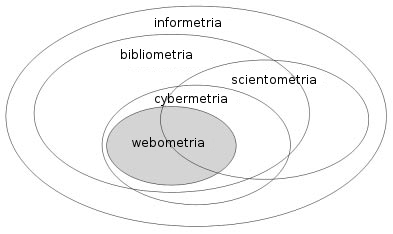
\includegraphics[width=\textwidth]{fields.png}
  \caption[Vzťah medzi jednotlivými disciplínami v~rámci informetrie]%
    {Diagram zobrazuje vzťah medzi disciplínami v~rámci informetrie .
    Bibliometria sa zaoberá publikáciami v~písomnej forme.
    Scientometria študuje vedecké publikácie v~písomnej forme ako aj
    ekonomické a sociálne vlastnosti vedy. Cybermetria analyzuje aspekty informácií
    na internete. Webometria skúma len web \citep{Bjorneborn2004}}.
  \label{fig:fields}
\end{figure}



Na Obrázku~\ref{fig:fields} vidíme, že informetria zahŕňa ostatné spomenuté
\uv{metrie,} pretože sa zaoberá skúmaním všetkých aspektov informácií.  Prienik
bibliometrie a scientometrie predstavuje použitie tých istých metód a zdrojov.
Naopak časť scientometrie, ktorá nezahŕňa bibliometriu vyjadruje sociálne a
ekonomické vlastnosti vedy. Webometria je úplne zahrnutá v bibliometrii,
pretože webové stránky sú komunikačné média, ktoré sú predmetom skúmania
bibliometrie.  Množina pre cybermetriu prečnieva z~bibliometrie, pretože sa
venuje aj iným komunikačným kanálom.

\section{Bibliometrické zákony}
\index{bibliometrické zákony|(}
\index{bibliometrický zákon|textbf}

\citet{Todeschini2016} definovali bibliometrický zákon (alebo taktiež nazývaný
informetrický zákon) ako matematický model, ktorý opisuje empirické závislosti
bibliometrických dát a javy ako distribúciu dokumentov v~istom súbore rôznych
autorov, alebo distribúciu citácií v~istom súbore dokumentov.  Bibliometrické
zákony sú generalizáciou istých štatistických dát.

V~období medzi rokmi 1920 a 1930 boli publikované tri hlavné bibliometrické
zákony: Lotkov zákon\index{Lotkov zákon}\index{bibliometrické zákony!Lotkov
  zákon} distribúcie vedeckých prác medzi autormi, Bradfordov zákon
\index{Bradfordov zákon}\index{bibliometrické zákony!Bradfordov zákon}
rozdelenia publikácií konkrétneho oboru vo vedeckých časopisoch a Zipfov
zákon\index{Zipfov zákon}\index{bibliometrické zákony!Zipfov zákon}
distribúcie slov v~texte \citep{Bellis2009}.


\subsection{Lotkov zákon}
\index{bibliometrické zákony!Lotkov zákon|textbf}
\index{Lotkov zákon|textbf}

Pomenovaný podľa amerického chemika, matematika a štatistika Alfreda J.\,Lotku.
Lotkov zákon opisuje frekvenciu publikačnej činnosti autorov v~danom obore.
\citet{Ondrisova2011} zhrnula obsah Lotkovej práce z~roku 1926, ktorej
v~definoval tento zákon.  Na začiatku zoradil autorov podľa počtu publikácií a
analyzoval aký počet prác prislúcha k~prvému autorovi, druhému atď.  Dáta čerpal
z~indexov \emph{Chemical Abstract} a \emph{Geschichtstafeln der Physik}.  Vyšla
mu jednoduchá matematická závislosť.  Počet autorov $f(n)$, ktorí publikovali
$n$ článkov v~danom obore ($n = 1, 2, 3, \dots$) sa blíži ku $1/n^2$ násobku
počtu autorov, ktorí publikovali jeden článok.

\citet{Egghe2005} definoval Lotkov zákon ako distribúciu vzťahom
(\ref{eq:lotka.law}), v~ktorom $K$ a~$\alpha$ sú kladné konštanty závisiace
na vedeckej oblasti.  Vo väčšine prípadov platí, že $\alpha = 2$ a $K = 1$.
\begin{equation}
\label{eq:lotka.law}
f(n) = \frac{K}{n^\alpha}
\end{equation}

Ak je známy počet autorov s~jedným článkom ($a_1$), je možné pomocou vzťahu
(\ref{eq:lotka.law2}) z~Lotkovho zákona určiť približný počet autorov s~$n$
publikáciami v~danom vedeckom obore.
\begin{equation}
\label{eq:lotka.law2}
a_n = \frac{a_1}{n^2}
\end{equation}
Napríklad v~súbore 100 autorov by štyria autori mali mať každý päť publikácii
($100/5^2 = 4$).


\subsection{Bradfordov zákon}
\index{bibliometrické zákony!Bradfordov zákon|textbf}
\index{Bradfordov zákon|textbf}

Britský knihovník Samuel Clement Bradford, si všimol istú pravidelnosť
v~distribúcii počtu článkov s~konkrétnou tématikou vo vedeckých časopisoch.
V~roku 1934 publikoval prácu, v~ktorej popísal tento jav
\citep{Bradford1985}\footnote{Pôvodný článok je v~súčasnosti nedostupný, ale
pre účely tejto práce sa odkazujeme na reprint z~roku 1985}.  V~danej vedeckej
práci študoval bibliografické záznamy časopisov z~oblasti geofyziky.  Články
týkajúce sa istej témy našiel v~326 časopisoch.  Potom zostupne usporiadal
časopisy podľa počtu článkov spadajúcich to danej témy.  Nakoniec ich rozčlenil
do troch skupín tak, aby každá skupina obsahovala zhruba taký istý počet
článkov:

\begin{itemize}
\item prvá skupina obsahovala 9 časopisov s~429 článkami,
\item druhá skupina obsahovala 59 časopisov s~499 článkami,
\item tretia skupina obsahovala 258 časopisov s~404 článkami.
\end{itemize}
Prvú skupinu, s~najväčším počtom článkov na časopis, pomenoval \emph{jadro},
druhú skupinu pomenoval \emph{prvá zóna} a tretiu skupinu pomenoval \emph{druhá
  zóna}.  Počty časopisov v~jednotlivých skupinách dal do pomeru:
\begin{equation*}
9 : 59 : 258 \;,
\end{equation*}
ktorý sa blíži k:
\begin{equation*}
9 : (9 \cdot 5) : (9 \cdot 5^2)
\end{equation*}
a mohol ho tak zjednodušiť na:
\begin{equation}
\label{eq:bradford.ration}
1 : 5 : 5^2
\end{equation}
Na základe výsledného pomeru (\ref{eq:bradford.ration}) definoval všeobecný
vzťah (\ref{eq:bradford.law}), známy ako Bradfordov zákon:
\begin{equation}
\label{eq:bradford.law}
1 : n : n^2 : \dotso \;,
\end{equation}
pričom $n$ sa nazýva Bradfordov násobok a je závislý od konkrétnych
bibliometrický dát.

Bradfordov zákon je považovaný za najlepší model vedeckého výskumu knižničnej a
informačnej vedy \citep[napr.][]{Nicolaisen2007}.


\subsection{Zipfov zákon}
\index{bibliometrické zákony!Zipfov zákon|textbf}
\index{Zipfov zákon|textbf}

Americký jazykovedec George Kingsley Zipf študoval kvantitatívnu analýzu jazyka
v~texte knihy Odyseus od Jamesa Joycesa. \citet{Powers1998} uvádza, že Zipf
vybral z~textu 29\,899 špecifických slov (vylúčil bežné slová ako
napr.\,predložky a spojky) a zoradil ich podľa frekvencie výskytu.  Prvé
najfrekventovanejšie slovo dostalo rang 1, druhé rang 2, atď.  Potom vynásobil
frekvenciu výskytu každého slova s~príslušným rangom.  Prekvapujúco mu vyšli
veľmi podobné hodnoty.Toto zistenie definoval matematicky vzťahom (\ref{eq:zipf.law}),
pričom $r$ je rang (poradové číslo) daného slova a $f$ je frekvencia výskytu
slova v~texte.  Tým pádom $c$ je konštanta, ktorá reprezentuje daný text.
\begin{equation}
\label{eq:zipf.law}
c = r \cdot f
\end{equation}
Paradoxne, Zipfov zákon neplatí iba v~lingvistike, ale je ho možné aplikovať
v~každej oblasti, kde sa skúma frekvencia výskytu konkrétneho javu.  Ako
napr.\,distribúcia počtu citácií, alebo návštevnosť webových stránok \citep{Li2002}.

\citet{Jiang2014} aplikovali Zipfov zákon na počty obyvateľov v~mestách.  V~najväčšom
meste je dvojnásobok počtu obyvateľov ako v~druhom najväčšom meste a trojnásobok
ako v~treťom najväčšom meste.

\index{bibliometrické zákony|)}


\section{Citačné registre}
\index{citačné registre|(}
\index{citačné registre|textbf}
\index{citačné indexy|see{citačné registre}}

Citačné registre (indexy) sú databázy, z~ktorých je možné vyhľadať citačné
odkazy na publikované odborné texty.  Ich analýzou je možné objektívne posúdiť
kvalitu citovaných publikácií.  Citačné registre vznikli preto, aby bolo možné
sledovať, aké ohlasy vo vedeckej komunite vzbudila daná publikácia.

Z~počiatku citačné indexy vychádzali v~tlačenej forme a ukladané boli ako
mikrofilmy.  S~príchodom nových elektronických médií sa k~nim pridali magnetické
pásky a nosiče CD-ROM.  Od rozšírenia internetu sú všetky citačné registre
prístupné on-line.


\subsection{Web of Science}
\index{citačné registre!Web of Science}
\index{Web of Science|textbf}
\index{WoS|see{Web of Science}}
\index{Web of Knowledge|see{Web of Science}}
\label{sec:wos}

\emph{Web of Science} (ďalej len WoS) je online platená služba umožňujúca prístup ku
citačným registrom a vykonať ich citačnú analýzu.  Poskytuje komplexné vyhľadávanie vo
viacerých citačných a abstraktových databázach, ktoré umožňuje dôkladne
scientometricky študovať medziodborové oblasti výskumu. \citet{Drake2005}
uvádza, že v~minulosti mala názov \emph{Web of Knowledge} a bola spravovaná
Inštitútom pre vedecké informácie \emph{Institute for Scientific Information}
(ISI).  V~súčasnosti je vo vlastníctve mediálneho gigantu \emph{Thomson Reuters}
so sídlom New Yorku, USA.

\citet{Smith2012} uviedol ako Eugene Garfield založil prvý moderný citačný
register.  Z~počiatku zahrňoval iba články venujúce sa genetike.  Neskôr v~roku
1960 založil inštitúciu \emph{Institute for Scientific Information} (ISI),
ktorá od nasledujúceho roku začala vydávať prvý \uv{Citačný index pre prírodné
vedy} \emph{Science Citation Index} (SCI), ktorý v~nasledujúcich rokoch začal
indexovať publikácie ostatných disciplín.  V~roku 1972 vznikol \uv{Citačný
index pre sociálne vedy} \emph{Social Science Citation Index} (SSCI) a
\uv{Citačný index pre umenie a humanitné vedy} \emph{Arts \& Humanities
Citation Index} (AHCI) v~roku 1978.

WoS zahrňuje viac než 50 000 odborných kníh, 12 000 časopisov a 160 000
príspevkov z~konferencií viacerých akademických oblastí od prírodných vied, cez
spoločenské vedy až po umenie.
\footnote{\url{http://wokinfo.com/citationconnection/realfacts}} Keďže súčasťou
WoS sú najstaršie citačné registre, tak obsahuje viac než 90 miliónov
bibliografických záznamov, ktoré majú viac než 800 miliónov citácií.
\footnote{\url{http://wokinfo.com/citationconnection}} Bohužiaľ väčšinu
databázy WoS tvoria záznamy z~amerických publikácií a konferencií. Pokrytie
dokumentov vydaných mimo Ameriky je obmedzené.  Čo samozrejme platí aj pre
citácie.

WoS pozostáva z~citačných registrov:\footnote{\url{http://wokinfo.com/products_tools/multidisciplinary/webofscience/}}

\begin{itemize}
\item \textbf{Science Citation Index Expanded\R\ (SCI-E):}\\
  Zahrňuje publikácie z~viac než 8\,500 časopisov, z~150
  vedeckých od oblastí roku 1900 do súčasnosti.
\item \textbf{Social Sciences Citation Index\R\ (SSCI):}\\
  Články z~viac než 3\,000 časopisov z~55 oblastí spoločenských vied a vybrané
  publikácie z~3\,500 vo svete vedeckých a technických
  časopisov od roku 1900 po súčasnosť.
\item \textbf{Arts \& Humanities Citation Index\R\ (A\&HCI):}\\
  Indexuje viac než 1\,700 časopisov z~oblasti umenia a humanitných vied a
  vybrané články z~viac než 250 časopisov z~oblasti spoločenských vied od roku 1975
  do súčasnosti.
\item \textbf{Index Chemicus\R\ (IC):}\\
  Obsahuje viac než 2,6 milióna záznamov zlúčenín od roku 1993 po súčasnosť.
\item \textbf{Current Chemical Reactions\R\ (CCR):}\\
  Zahrňuje viac než milión chemických reakcií od roku 1986, plus záznamy
  z~francúzskeho Inštitútu duševného vlastníctva (INPI) od
  roku 1840 do 1985.
\item \textbf{Book Citation Index\R\ -- Science (BKCI-S) a Book Citation
  Index\R\ -- Social Sciences \& Humanities (BKCI-SSH):}\\
  Poskytuje viac než 60\,000 vybraných kníh.  Od roku 2005 pribúda 10\,000 nových kníh
  každým rokom.
\item \textbf{Conference Proceedings Citation Index\R\ -- Science (CPCI-S) a
  Conference Proceedings Citation Index\R\ -- Social Sciences \& Humanities
  (CPCI-SSH):}\\ Zahrňuje príspevky z~viac než 160\,000 konferencií z~256
  rôznych oblastí \uv{vedy a techniky (CPCI-S)} a \uv{sociálnych a
  humanitných vied (CPCI-SSH)} od roku 1990.  Každým rokom do nej pribúda
  takmer 400\,000 konferenčných príspevkov z~cca.\,12\,000 konferencií.
\end{itemize}


Okrem citačného registru \emph{Web of Science}, \emph{ISI Web of Knowledge}
obsahuje nástroje na jednoduchý prístup k~publikáciám a ich citačnej
analýze: \footnote{\url{http://thomsonreuters.com/content/dam/openweb/documents/pdf/scholarly-scientific-research/fact-sheet/wos-next-gen-brochure.pdf}}


\begin{itemize}
\item \textbf{Journal Citation Reports:} Poskytuje systematické a objektívne
  hodnotenie svetových časopisov a ich vzájomné porovnanie použitím metrík ako
  impakt faktor.
\item \textbf{Essential Scientific Indicator:} Umožňuje analyzovať a hodnotiť
  vedecký výkon spoločností, inštitúcií, krajín a časopisov.
\item \textbf{InCites:} Komplexný nástroj, ktorý umožňuje akademickým,
  alebo vládnym pracovníkom hodnotiť inštitúcie na základe počtu citácií.
\item \textbf{Converis:} Je manažérsky nástroj pre univerzity, a iné vedecké
  inštitúcie.
\item \textbf{ScholarOne:} Je manažérsky systém pre vydavateľov vedecký
  publikácií ako časopisov, kníh a zborníkov z~konferencií. Umožňuje
  manažovať príspevky, \uv{peer review} proces a samotnú publikáciu.
\item \textbf{EndNote:} Poskytuje manažovať vlastné publikácie a umožňuje
  ich bibliometrickú analýzu.
\end{itemize}



\subsection{Scopus}
\index{citačné registre!Scopus|textbf}
\index{Scopus|textbf}
\label{sec:scopus}

Scopus\,\R je citačný register európskeho vydavateľstva \emph{Elsevier} so sídlom
v~Amsterdame, Holandsko.  Jedná sa o~platenú službu, rovnako ako WoS.  Bol
spustený v~novembri 2004, ale retrospektívne obsahuje záznamy od roku 1996.
Scopus obsahuje viac záznamov hlavne z~oblasti Európy.  Okrem časopisov obsahuje
aj zborníky, patenty a webové sídla.  Aktualizuje sa denne.  Podľa údajov
z~januára 2016 indexuje viac ako 21\,500 titulov, ktoré zahrňujú:

\begin{itemize}
  \item viac než 21\,500 recenzovaných časopisov (z~toho 4\,200 prístupných
    zdarma),
  \item viac než 360 obchodných časopisov,
  \item viac než 530 knižných edícií,
  \item viac než 7,2 milióna konferenčných príspevkov z~83\,000 konferencií,
  \item viac než 116\,000 knižných titulov,
  \item viac ako 27 miliónov patentových záznamov z~piatich patentových úradov,
  \item články v~tlači (Articles-in-Press) z~viac ako 5\,000 časopisov.
\end{itemize}

Databáza k~januáru 2016 obsahuje viac než 60 miliónov záznamov v~jadre, z~toho:\footnote{\url{https://www.elsevier.com/__data/assets/pdf_file/0007/69451/scopus_content_coverage_guide.pdf}}

\begin{itemize}
  \item viac než 38 miliónov záznamov od roku 1996 (84\,\% všetkých citácií),
  \item viac než 22 miliónov záznamov z~obdobia 1823--1995 (staršie záznamy
    obsahujú len abstrakty bez citácií),
  \item okolo 3 milióna záznamov pribúda každým rokom (5\,500 za deň).
\end{itemize}

V~decembri 2015 bolo pridaných viac než 93 milióna citácií na viac než päť
miliónov článkov starších z~pred roku
1996.

\subsection{Google Scholar}
\index{citačné registre!Google Scholar|textbf}
\index{Google Scholar|textbf}
\index{GS|see{Google Scholar}}
\label{sec:gs}

Google Scholar \footnote{\url{https://scholar.google.com/}} (ďalej len GS) je neplatená online
služba, ktorá bola spustená v~roku 2004.  Umožňuje vyhľadávať bibliografické
záznamy z~databázy GS. Na rozdiel od WoS a \emph{Scopusu}, ktoré sú obmedzené
len na istej skupiny konkrétnych vydavateľstiev, alebo časopisov, GS indexuje
plné texty a metadáta databáz vydavateľov odbornej literatúry, odborných
časopisov, archívov, ktoré obsahujú preprintové a voľnoprístupné (open access)
dokumenty, záverečné práce, patenty a webové stránky. Všetky dokumenty, ktoré
\uv{pôsobia} vedecky \citep{Vine2006}.  Projekt Google Book je tiež indexovaný
s~GS.  Síce Google nikdy nezverejnil rozsah databázy Google Scholar, ale
\citet{Orduna-Malea2015} určili veľkosť na takmer 160 miliónov dokumentov k~máju
2014. \citet{Khabsa2014} zistili, že GS zahrňuje 87\,\% anglicky písaných
dokumentov, na vzorke 114 miliónov dokumentov.

Bibliografické záznamy sú automaticky generované analýzou indexovaných
dokumentov \citep{Vine2006}. Čo spôsobuje mnohé chyby nie len u~citovaných, ale
aj citujúcich záznamoch. Najčastejšie chyby sú:
\begin{itemize}
  \item \emph{Duplicitné záznamy} vznikajú stiahnutím bibliografických záznamov
    na rovnaký dokument z~viacerých zdrojov (napr. vydavateľ a databáza abstraktov).
  \item \emph{Nekompletné záznamy} najčastejšie neobsahujú rok publikácie,
    alebo názov publikácie je nekompletný, či dokonca chýba.  Veľmi častým
    javom je vloženie časti listu autorov do názvu publikácie, či dokonca ho
    úplne nahradí.  Túto chybu je možné jednoducho korigovať, pretože väčšina
    záznamov obsahuje internetovú adresu zdroja. Problém nastáva, ak neobsahujú
    internetový odkazu na zdroj, ktoré sú označené ako \texttt{[CITATION]}.
    Tento fakt komplikuje ručnú korekciu, pretože je potrebné danú publikáciu
    vyhľadať, čo nie vždy je možné.
  \item \emph{Neúplný list autorov} je vlastnosť GS. Vždy vyberá max 5 autorov,
    ale vyskytuje sa záznam, ktorý neobsahuje vyhľadávané meno, alebo neobsahuje
    žiadnych autorov.
  \item \emph{Analýza nesprávnych dokumentov} vzniká pretože žiadny algoritmus nie je
    dokonalý.  Najčastejšie indexuje zoznam autorov v~zborníku ako samostatný
    dokument, alebo ak zadané meno autora je bežné slovo (napr. Lesný).  Niekedy
    indexu dokument, ktorý vôbec nesúvisí s~kľúčom vyhľadávania.
    GS dokonca spojil zoznam autorov so zbytkom referencie z~ďalšieho článku zo
    zoznamu referencií.
\end{itemize}

\noindent Webové rozhranie umožňuje základné vyhľadávanie podľa názvu, autorov a
časopisu.  Výsledkom je zoznam publikácií s~počtom citácií, ktorý je rangovaný
podľa počtu citácií a slov v~názve \citep{Beel2009}.  Ďalšie usporiadanie je
možné iba podľa dátumu.  Filtrovať výsledky je možné len podľa roku, alebo či
je to patent.  Vo výsledkoch hľadania je názov publikácie odkazom na zdroj
záznamu (odkaz chýba ak sú označené ako (\texttt{[CITATION]}). \emph{Cited by}
je odkaz na zoznam citujúcich dokumentov.  Odkazom \emph{Related articles} sa
vytvorí zoznam dokumentov z~rovnakej oblasti.  Funkcia \emph{Metrics} umožňuje
hodnotenie časopisov podľa $h$-indexu za päť rokov, alebo mediánu citácií na
h-core články. V~časopisoch je možné vyhľadávať a zoraďovať podľa disciplíny a
krajiny.  Obmedzenia webového rozhrania môžu riešiť externé softvérové aplikácie.

Často používanou externou aplikáciou na~získanie a spracovanie scientometrických
dát je program \emph{Publish or Perish}\index{Publish or Perish|textbf} (ďalej
len PoP).  Program umožňuje priamo získať dáta z~citačných registrov GS a
Microsoft Academic\footnote{\url{https://academic.microsoft.com}} a importovať
dáta zo súboru, ktorý bol exportovaný z~citačných registrov WoS a Scopus.  Dáta
je možné exportovať do rôznych formátov (napr. CSV\footnote{Formát textového
súboru, ktorý obsahuje tabuľku dát. Jednotlivé riadky súboru zodpovedajú
riadkom tabuľky a položky jednotlivých stĺpcoch sú oddelené čiarkou a prípadne
ohraničené úvodzovkami.  Názov formátu pochádza z~ang. \emph{comma-separated
values}.} alebo Microsoft Excel) a dodatočne spracovať. Taktiež má
v~dispozícii mnoho citačných indexov na scientometrické zhodnotenie dát
\citep{Harzing2011}.

Už od spustenia GS prijal veľa kritiky.  Generovaním bibliografických záznamoch
s~chybami \citep{Jacso2009,Jacso2010}.  GS dáva možnosť umelo zvyšovať kredit
istých článkov či už publikovaním autocitácií v~nekarentovaných časopisoch
modifikáciou a ďalšou publikáciou vlastných článkov \citep{Beel2010b},
generovaním nezmyselných článkov programe \emph{SCIgen}\index{SCIgen|textbf}
\footnote{Program SCIgen vygeneruje dokument, ktorý formálne pôsobí ako
vedecká publikácia zadaných autorov z~oblasti informatiky, ale obsah nemá
žiadny zmysel \citep{Labbe2013};\\\url{https://pdos.csail.mit.edu/archive/scigen/}}

\citep{Beel2010a}.
Keďže z~princípu fungovania GS by mal pokrývať publikácii, zdá sa to ako
ideálny zdroj bibliometrických dát.  Skutočnosť je však úplne opačná. Databáza
stále nepokrýva 100\,\% publikácií v~štandardných citačných registroch (ako WoS
a Scopus). Publikácie v~malých časopisoch, ktoré nie sú indexované vo WoS a Scopus,
majú minimum citácií (väčšinou žiadne). Pokiaľ tieto časopisy sú silno citované,
väčšinou je to dôsledok cielenej manipulácie.  Výskyt chybných bibliografických
záznamov bez prácnej ručnej korekcie dáva iba približný, informatívny, účel a
preto musia byť brané s~rezervou.

\index{citačné registre|)}

\section{Citačné indikátory}
\index{citačné indikátory|(}
\index{citačný indikátor|textbf}
\label{sec:indicators}

Citačný indikátor je druh scientometrickej metódy na stanovenie \uv{kvality}
vedeckých publikácii, vedeckých pracovníkov a vedeckých inštitúcii.  Všetky
indexy vychádzajú zo základných scientometrických parametrov: počet publikácii a
množstvo ich citácii.  Pri výpočte niektorých indexov zohľadňujú aj iné
parametre (napr.\,vek pracovníkov).

Základným indikátorom je citačná frekvencia, t.\,j.\,priemer počtu citácií istej
skupiny publikácií v~danom obore za určitý
rok.\footnote{\url{http://ipscience-help.thomsonreuters.com/incitesLiveESI/ESIGroup/fieldBaselines/
citationRatesBaselines.html}}

Ešte nikto nevymyslel citačný indikátor, ktorý je schopný objektívne obsiahnuť
všetky scientometrické aspekty vedy. Preto bolo ich vytvorené veľké množstvo a
stále sa tvoria nové. Každý je určený na hodnotenie iného aspektu a na
komplexnú kvalitatívnu analýzu je potrebné zvoliť ich správnu kombináciu.

\subsection{Prehľad citačných indikátorov}

Pre účely tejto práce sme zvolili citačné indikátory uvedené v~Tabuľke
\ref{tab:indicators.review}, pretože sú kombináciou najpoužívanejších citačných
indikátorov na hodnotenie časopisov (\emph{journal citation indikators}) a
citačných indikátorov, ktoré využíva program PoP\index{Publish or Perish}.
Práve takéto rozčlenenie citačných indikátorov do podkapitol sme použili
v~tejto práci.

Tabuľka \ref{tab:indicators.review} predstavuje prehľad citačných indikátorov
použitých v~tejto práci. Takmer všetky slovenské názvy vznikli prekladom
anglického pomenovania (okrem CiteScore a $AW$-index, ktoré sa neprekladajú do
slovenčiny).  V~slovenskej literatúre je to už zaužívané \emph{Journal Impact
Factor} prekladať len ako impact faktor.  Pomocou anglického názvu je
jednoduché vyhľadať všetky informácie o~danom citačnom indikátore v~zahraničnej
literatúre. Skratky používame v~texte tejto práce a zároveň sa bežne používajú
v~zahraničnej literatúre. Symboly sa vyskytujú iba v~matematických vzorcoch.
U~niektorých indikátorov chýba matematický symbol, z~dôvodu výskytu len slovnej
definície v~texte, alebo matematická definícia nie je v~tejto práci uvedená
(uvedenie definície je pre komplikovanosť nad rámec rozsahu tejto práce).

Najčastejšie používaný citačný indikátor na hodnotenie časopisov je impakt faktor, a~to
jednak z~historických dôvodov a tiež kvôli jednoduchosti výpočtu. CiteScore, SciMago a
SNIP sa používajú na hodnotenie časopisov z~citačného registru Scopus.
Z~ostatných je to bezvýhradne Hirshov index, pretože je najstarší, ale Eggheov
index je tiež veľmi používaný.  Ostatné sa využívajú na hodnotenie špecifických
scientometrických aspektov vedy.

Jednotlivé citačné indikátory budú v~tejto práci podrobnejšie
rozvedené (viď posledný stĺpec Tabuľky \ref{tab:indicators.review})

\begin{table}
  \caption[Prehľad citačných indikátorov]%
  {Prehľad citačných indikátorov, ktoré sme použili v~tejto práci. Rozdelili sme
    ich na citačné indikátory, ktoré na používajú na hodnotenie časopisov
    (označ.\,$^\dagger$) a ostatné. Tabuľka obsahuje ich skratku a tiež symbol,
    ktorým sa označujú v~matematických vzorcoch a tabuľkách. Posledný stĺpec
    \uv{Kap.} obsahuje číslo podkapitoly tejto práce, kde sú jednotlivé citačné
    indikátory podrobne vysvetlené. PoP je skrátený názov programu
    \emph{Publish or Perish}.}
  \label{tab:indicators.review}
  \centering\small
  \begin{tabularx}{\textwidth}{llccr}
    \toprule
    Slovenský  názov & Anglický názov & Skratka & Symbol & Kap. \\
    \midrule
    impakt faktor$^\dagger$         & \emph{Journal Impact Factor}           & IF                  & $\mathit{IF}$     & \ref{sec:if}        \\[0.5ex]
    SciMago rang časopisu$^\dagger$ & \emph{SciMago Journal Rank}            & SJR                 & --                & \ref{sec:sjr}       \\[0.5ex]
    CiteScore$^\dagger$$^\ddagger$    & \emph{CiteScore}                       & --                  & --               & \ref{sec:citescore}  \\[0.5ex]
    normalizovaný impakt           & \emph{Source normalized impact}        & SNIP                & --                & \ref{sec:snip}      \\[-0.25ex]
    časopisu  na dokument$^\dagger$  & \emph{per paper}                       &                     &                   &                     \\[0.5ex]
    Hirschov index                 & \emph{Hirsh's index}                   & $h$-index           & $h$                & \ref{sec:h-index}  \\[1.5ex]
    Eggheov index                  & \emph{Egghe's index}                   & $g$-index           & $g$                & \ref{sec:g-index}  \\[0.5ex]
    Zhangov $e$-index              & \emph{Zhang's $e$-index}               & $e$-index           & $e$                & \ref{sec:e-index}  \\[0.5ex]
    súčasný $h$-index              & \emph{Contemporary $h$-index}          & $h^{\mathrm{c}}$-index & $h^{\mathrm{c}}$     & \ref{sec:hc-index}  \\[0.5ex]
    citačná frekvencia váhovaná    & \emph{Age-weighted citation rate}      & AWCR                 & --                & \ref{sec:aw-index} \\[-0.25ex]
    podľa veku                     &                                        &                      &                   &                    \\[0.5ex]
    $AW$-index$^\ddagger$            & \emph{$AW$-index}                      & $AW$-index           & $\mathit{AW}$     & \ref{sec:aw-index} \\[1.5ex]
    pôvodný individuálny $h$-index & \emph{Individual $h$-index (original)} & $h_{\mathrm{I}}$-index  & $h_{\mathrm{I}}$     & \ref{sec:hi-index} \\[0.5ex]
    variant individuálneho        & \emph{Individual $h$-index}            & $h_{\mathrm{I,norm}}$    & $h_{\mathrm{I,norm}}$ & \ref{sec:hinorm}   \\[-0.25ex]
    $h$-indexu pre PoP             & \emph{(PoP variation)}                 &                      &                   &                    \\[0.5ex]
    multiautorský $h$-index        & \emph{Multi-authored $h$-index}        & $h_{\mathrm{m}}$-index  & $h_{\mathrm{m}}$     & \ref{sec:hm-index} \\
    \bottomrule \\ [-2ex]
    \multicolumn{5}{l}{\footnotesize $^\dagger$ citačné indikátory na hodnotenie časopisov} \\
    \multicolumn{5}{l}{\footnotesize $^\ddagger$ indikátory, ktorých názov sa neprekladá so slovenčiny}
  \end{tabularx}
\end{table}


\section{Citačné indikátory na hodnotenie časopisov}

\subsection{Journal Impact Factor (IF)}
\index{citačné indikátory!journal impact factor@\emph{journal impact factor}|textbf}
\index{journal impact factor@\emph{journal impact factor}|textbf}
\label{sec:if}

Prvý citačný indikátor navrhol zakladateľ citačných registrov
\citet{Garfield1955} ako presnejší spôsob evaluácie autorov vedeckých článkov
než v~tej dobe používané počty publikácií a počty citácií.

V~súčastnosti IF používa \emph{Institute of Scientific Information} na
každoročné hodnotenie vedeckých časopisov v~rámci \emph{Journal citation
reports} (JCR).  Impact Factor je priemerný počet citácií na články a
prehľadové články publikované v~danom časopise za posledné dva roky.

Impact Factor pre rok 2016 možno matematicky vyjadriť vzťahom (\ref{eq:if}),
kde $a$ je celkový počet článkov a prehľadových článkov, ktoré boli v~danom
časopise publikované v~rokoch 2014--2015 a $c$ je počet článkov publikovaných
v~danom časopise v~rokoch 2014--2015, ktoré boli citované v~publikáciach
indexovaných v~roku 2016.\footnote{Výsledný Impact Factor z~roku 2016 môže byť
publikovaný až v~roku 2017, pretože ho nie je možné vypočítať skôr, než rok
2016 skončí.}

\begin{equation}
\label{eq:if}
\mathit{IF}_{2016} = \frac{c}{a}
\end{equation}

\noindent JCR poskytuje IF za päťročné obdobie.\footnote{\url{http://admin-apps.webofknowledge.com/JCR/help/h_impfact.htm}}

\subsection{SciMago Journal Rank (SJR)}
\index{citačné indikátory!SciMago Journal Rank|textbf}
\index{citačné indikátory!SJR|see{SciMago Journal Rank}}
\index{SciMago Journal Rank|textbf}
\index{SJR|see{SciMago Journal Rank}}
\label{sec:sjr}

SCImago Journal Rank (skrátene SJR) je indikátor na hodnotenie vplyvu
vedeckých časopisov. Používa sa ako alternatíva k~už spomínanému impakt faktoru
\citep{Falagas2008}.  Na rozdiel od IF, ktorý na výpočet používa len počet prijatých
citácií, SJR berie do úvahy aj prestíž zdrojov, z~ktorých citácie pochádzajú.
Proces výpočtu prestíže časopisov \citep{GuerreroBote2012} je inšpirovaný algoritmom
Google PageRank\texttrademark{} \citep{Page1999}.

SJR je každoročne vypočítavaný pre viac než 21\,500 titulov od viac než 5\,000
medzinárodných vydavateľstiev.
\footnote{\url{http://www.scimagojr.com/aboutus.php}} Citačné dáta sú čerpané
z~citačného registru Scopus \textregistered. Oficiálne stránky
\footnote{\url{http://www.scimagojr.com}} umožňujú rangovať časopisy v~27
hlavných kategóriách, 313 podkategóriách, alebo podľa štátu.  Taktiež poskytuje
rangovanie štátov podľa tzv.\,SCImago Country Rank.  Webový portál a služby
spravuje SCImago výskumná skupina Consejo Superior de Investigaciones
Científicas (CSIC), Granadská univerzita, Extremadura, Carlos III (Madrid).


\subsection{CiteScore}
\index{citačné indikátory!CiteScore|textbf}
\index{CiteScore|textbf}
\label{sec:citescore}

8. decembra 2016 vydavateľský gigant Elsevier (vlastník citačného registru
Scopus) spustil nový index na scientometrické hodnotenie časopisov.  CiteScore
pre rok 2015 je matematicky definovaný vzťahom (\ref{eq:citescore}), kde $B$
je celkový počet publikácií, ktoré boli publikované v~danom časopise v~rokoch
2012-2014 (trojročné obdobie) a $A$ je počet citácií, ktoré tieto články
získali v~roku 2015
\footnote{\url{https://journalmetrics.scopus.com/downloads/CiteScoreMetrics_FAQ_Scopus_Dec2016_LO.pdf}}.

\begin{equation}
\label{eq:citescore}
CiteScore\; 2015 = \frac{A}{B}
\end{equation}

Na rozdiel od impakt faktoru, CiteScore je možné získať priamo sa stránkach
indikátorov pre časopisy od
Scopusu\footnote{\url{https://journalmetrics.scopus.com}}, kde sa dozvieme
ďalšie informácie ako počet dokumentov, počet citácií, ktoré v~prípade IF sú
prístupné iba predplatiteľom.  Navyše k~informáciám o~časopise sú pridané
informácie ako CiteScore rang percento, citovaných dokumentov, SJR a SNIP.
Portfólio CiteScore zahrňuje viac než 22\,000 časopisov, čo je približne o~11\,000
viacej než portfólio IF
\footnote{\url{https://www.elsevier.com/__data/assets/pdf_file/0006/239046/CiteScoreMetrics_Factsheet_Elsevier_Dec2016_LO.PDF}}.

Najväčším rozdielom medzi IF a CiteScore je druh dokumentov, ktoré sa
započítavajú do výpočtu. Oproti IF, kde sa započítavajú len tzv.\,citovateľné
dokumenty ako článok a prehľadový článok (ktoré sú väčšinou najcitovanejšie).
Pri výpočte CiteScore sa započítavajú \emph{všetky} publikácie vrátane tzv.
necitovateľných dokumentov, ako napr. príspevky z~konferencií, editoriál, listy
a diskusné príspevky (ktoré dostávajú minimum citácií), pre čo je ostro
kritizovaný
\footnote{\url{https://scholarlykitchen.sspnet.org/2016/12/12/citescore-flawed-but-still-a-game-changer/}}.
Prestížne časopisy ako \emph{The Lancet}, \emph{Nature} a \emph{Science}
získali priemerný CiteScore rang, čo sa prisudzuje najmä zahrnutím
necitovateľných dokumentov.

Vedci z~projektu Eigenfactor z~Washingtonskej univerzity v~Seattle zistili, že
časopisy publikované Elsevierom majú priemere o~25\,\% vyššiu hodnotu CiteScore
oproti impact faktoru
\footnote{\url{http://eigenfactor.org/projects/posts/citescore.php}}. Príčinou
tohoto fenoménu je, že Elsevier publikuje časopisy, ktoré obsahujú minimum
necitovateľných dokumentov.

Vyskytli sa chyby v~zaraďovaní časopisov do odborov. Napríklad časopis \emph{Annual
Review of Plant Biology} (ročenka z~oblasti biológie rastlín) získal štvrté miesto
z~v~oblasti všeobecnej medicíny.

I~napriek vyššie uvedeným problémom je CiteScore prijímaný ako konkurencia impakt faktoru.

%\subsubsection{Normalizovaný impakt časopisu na dokument (Source normalized impact
%per paper -- SNIP)}
\subsection{Normalizovaný impakt časopisu na dokument (SNIP)}
\index{citačné indikátory!Normalizovaný impakt časopisu na
dokument|textbf}
\index{Normalizovaný impakt časopisu na dokument|textbf}
\index{SNIP|see{Normalizovaný impakt časopisu na dokument}}
\label{sec:snip}

Je známe, že časopisy rôznych oborov sa líšia v~citačnom štandarde.  Napríklad
medicínske časopisy majú vždy väčší počet citácií ako časopisy z~oblasti
scientometrie. Citačný štandard závisí od mnoho faktorov, ako napr.  celkový
počet ľudí pracujúcich v~obore, distribúcia typu článku (štúdia, metóda,
prehľad).  Tým pádom nie je vhodné porovnávať časopisy z~rôznych disciplín len
na základe počtu citácií, resp. indexov, ktoré zahŕňajú iba absolútny počet
citácií (IF, CiteScore).  Preto \citet{Moed2010} navrhol nový indikátor na
hodnotenie časopisov: normalizovaný impakt časopisu na dokument (\emph{Source
normalized impact per paper}), skr. SNIP. Definoval ho ako pomer medzi počtom
citácií na publikáciu v~danom časopise a tzv.\,citačný potenciál (priemerný
počet citácií na jednu publikáciu v~danom obore).

\citet{Waltman2013} upravili Moedov SNIP. Pri výpočte citačného potenciálu
nahradili aritmetický priemer, ktorý navrhol Moed, za harmonický priemer.
Centrum pre vedecké a technologické štúdie, Univerzity v~Leidene, Holandsko
\footnote{\url{http://www.journalindicators.com/}} každoročne počíta SNIP pre
viac než 20\,000 svetových časopisov.  Dáta získavajú z~citačného registru
\emph{Scopus}. V~súčasnosti sa spolu s~SJR a CiteScore uvádza aj SNIP pre daný
časopis.

\section{Ostatné citačné indikátory}

\subsection{Hirschov index ($h$-index)}
\index{citačné indikátory!Hirshov index|textbf}
\index{citačné indikátory!h-index@$h$-index|see{Hirshov index}}
\index{Hirshov index|textbf}
\index{h-index@$h$-index|see{Hirshov index}}
\label{sec:h-index}

Tento populárny citačný indikátor bol definovaný Jorgem E.\,Hirshom v~roku 2005
ako číslo $h$, ktoré zodpovedá počtu najcitovanejších článkov daného autora,
ktorých každá publikácia má aspoň $h$ citácii \citep{Hirsch2005}.

Pre lepšie pochopenie je vhodné uviesť príklad: Vedec A~má 10 publikácii.  Ak
ich zoradíme podľa počtu citácii, potom prvá má 10 citácii, druhá má 8, tretia
5, štvrtá 4, piata 2 a ostatné nemajú žiadne citácie.  Potom tento vedec má
$h$-index 4, pretože štyri najcitovanejšie články (s~počtami citácii 10, 8, 5 a
4) majú aspoň po 4 citácie. Skupina článkov, z~ktorých každý má aspoň toľko citácií,
ako je hodnota $h$-indexu sa súhrne nazýva h-core články.\index{h-core články|textbf}

Hlavným problémom $h$-indexu je necitlivosť na malý počet veľmi citovaných článkov
(Napríklad ak porovnáme publikačnú činnosť vedca A~s~predchádzajúceho príkladu
s~vedcom B, ktorý má iba 5 publikácií so 108, 45, 12, 5 a 2 citáciami, jeho
Hirshov index je rovnaký ako vedca A.

Sám Hirsh uviedol, že $h$-index nemožno použiť na porovnávanie autorov rôznych
vedných disciplín.


\subsection{Eggheov index ($g$-index)}
\index{citačné indikátory!Eggheov index|textbf}
\index{citačné indikátory!g-index@$g$-index|see{Eggheov index}}
\index{Eggheov index|textbf}
\index{g-index@$g$-index|see{Eggheov index}}
\label{sec:g-index}

Leo Egghe \citeyearpar{Egghe2006} publikoval indikátor $g$-index, ktorý má vyriešiť niektoré
problémy $h$-indexu, najmä jeho necitlivosť k~autorom, ktorí majú málo extrémne
citovaných publikácii.

Eggheov $g$-index je definovaný ako číslo $g$, ktoré predstavuje počet
najcitovanejších článkov konkrétneho autora, zostupne zoradený podľa počtu
citácií, ktorého druhá mocnina je menšia alebo rovná súčtu všetkých citácií
daných článkov.

Napríklad ak má vedec A~desať publikácií, ktoré majú 6, 6, 5, 4, 2, 0, 0, 0, 0 a
0 citácií.  Jeho $h$-index je 4 a $g$-index je 4.
($6+6+5+4 = 21 \geq 4\cdot4=16$) Vedec B má šesť publikácií s~15, 10, 5, 4, 3 a
2 citáciami.  Aj jeho $h$-index je tiež 4, ale $g$-index je 6.
($15+10+5+4+3+2 = 39 \geq 6\cdot6 = 36$)

Ako je z~príkladu zrejmé, $g$-index $\geq$ $h$-index.  Keďže $g$-index berie do
úvahy viacej citácií, ale stále je necitlivý ku autorom malého počtu extrémne
citovaných článkov.  Pokiaľ vedec má napr.\,10 publikácií, ktoré sú spolu 300
citované, tak jeho maximálny $g$-index je 10 a zvyšných 200 citácií je
ignorovaných.  Z~toho dôvodu sám Egghe navrhol umelo zvýšiť počet článkov na
číslo $T$, ktorého druhá mocnina sa blíži ku celkovému počtu citácií
\citep{Egghe2006}.  Samozrejme manipulovanie s~dátami nie je dobrá metóda a
preto je potrebné použiť iný indikátor, ktorý je schopný zachytiť podobné
prípady.


\subsection{Zhangov $e$-index}
\index{citačné indikátory!Zhangov e-index@Zhangov $e$-index|textbf}
\index{citačné indikátory!e-index@$e$-index|see{Zhangov $e$-index}}
\index{Zhangov e-index@Zhangov $e$-index|textbf}
\index{e-index@$e$-index|see{Zhangov $e$-index}}
\label{sec:e-index}

Ako reakciu na malú citlivosť $h$-index a $g$-indexu pre autorov s~malým
množstvom veľmi citovaných prác \citet{Zhang2009} navrhol nový indikátor
$e$-index.  Zhang ho definoval ako číslo $e$, ktoré je druhou odmocninou
rozdielu všetkých citácií h-core článkov a maximálnym počtom citácií, ktoré sú
zahrnuté do $h$-indexu $h^2$.

Napríklad, ak $h$-index akademického pracovníka je 10 a jeho publikácie v~h-core
majú spolu 200 citácií, tak jeho $e$-index bude 10, pretože ak odčítame
teoretické minimum na dosiahnutie $h$-indexu 10, t.\,j.\,100 citácii od skutočného
počtu citácii h-core článkov 200, výsledok bude 100, z~čoho druhá odmocnina je
10.

To znamená, že $e$-index možno použiť na odlíšenie dvoch vedcov s~rovnakým
$h$-indexom, ale rozdielnou citačnou frekvenciou.


\subsection{Súčasný $h$-index (Contemporary $h$-index)}
\index{citačné indikátory!súčasný h-index@súčasný $h$-index|textbf}
\index{súčasný h-index@súčasný $h$-index|textbf}
\index{contemporary h-index@\emph{contemporary $h$-index}|see{súčasný $h$-index}}
\label{sec:hc-index}

Autori citačných indikátorov si uvedomujú že vedecká literatúra starne.
Všeobecne vedecká práca z~pred 10 rokov má menší impakt, ako rok stará
publikácia s~rovnakým množstvom citácií.  Sám \citet{Hirsch2005} navrhol
tzv.\,m-kvocient, čo nie je nič iné ako h-index podelený počtom rokov od vydania
prvej práce daného vedca.  Teda výrazne nezvýhodňuje starších akademikov, bez
ohľadu na to, či sú stále aktívni, a citovanosť ich najnovších publikácií.

Z~toho dôvodu \citet{Sidiropoulos2007} navrhli indikátor, ktorý zahrňuje vek
jednotlivých článkov.  Pomenovali ho Súčasný (contemporary) $h$-index\,--\,$h^{\mathrm{c}}$,
ktorý definovali:

\uv{Vedec má $h^{\mathrm{c}}$ ak každý jeho článok z~množiny
  $\mathrm{N_p}$ dosiahne skóre $S^{\mathrm{c}}(j) \geq h^{\mathrm{c}}$ a ostatné
  články $(\mathrm{N_p} - h^{\mathrm{c}})$ dosiahli skóre
  $S^{\mathrm{c}}(j) \geq h^{\mathrm{c}}$.}

Skóre $S^{\mathrm{c}}(j)$ je definované vzťahom (\ref{eq:hc-index.score}), pričom $Y(j)$
predstavuje rok, kedy bol článok $j$ publikovaný a $\mathit{cit}_j$ znamená jeho
maximálny počet citácií.

\begin{equation}
\label{eq:hc-index.score}
S^{\mathrm{c}}(j) = \gamma\cdot (Y(\mathrm{teraz}) - Y(j) + 1)^{-\delta}\cdot \mathit{cit}_j
\end{equation}

Pri nastavení $\delta = -1$ sa dosiahne, že počet citácií daného článku je
podelený jeho vekom v~rokoch.  Lenže, podľa autorov, podelením počtu citácií
daného článku jeho vekom sa získajú príliš malé hodnoty skóre
$S^{\mathrm{c}}(j)$ na dosiahnutie reprezentatívneho $h$-indexu.  Preto autori
zaviedli koeficient $\gamma$, ktorý podľa empirickej štúdie autorov je
najvýhodnejšie  nastaviť na $\gamma = 4$.

%\subsection{Citačná frekvencia váhovaná podľa veku (Age-weighted citation rate
%  -- AWCR) a $\mathit{AW}$-index}
\subsection{Citačná frekvencia váhovaná podľa veku (AWCR) a $\mathit{AW}$-index}
\index{citačné indikátory!cit. frekvencia váhovaná podľa veku|textbf}
\index{citačné indikátory!AW-index@$\mathit{AW}$-index|see{citačná frekvencia váhovaná podľa veku}}
\index{citačná frekvencia váhovaná podľa veku|textbf}
\index{AW-index@$\mathit{AW}$-index|see{citačná frekvencia váhovaná podľa veku}}
\index{age-weighted citation rate@\emph{age-weighted citation rate}|see{citačná frekvencia váhovaná podľa veku}}
\index{AWCR|see{citačná frekvencia váhovaná podľa veku}}
\label{sec:aw-index}

Vek vedeckej publikácie (rozdiel medzi dnešným rokom a rokom vydania daného
článku) sa považuje za jeden z~faktorov, ktorý definuje impakt článku.  Na jeho
kvantifikáciu je nutné započítať tento parameter do výpočtu.  Jednoduchým
delením počtu citácií danej publikácie jej vekom váhujeme citačnú frekvenciu
podľa veku publikácie (ang. \emph{age-weighted citation rate}, skr. AWCR).

\citet{Jin2007} vytvorili indikátor, ktorý váhuje citačnú frekvenciu h-core
článkov podľa veku.  Nazvali ho $\mathit{AR}$-index.

Jeho matematická definícia je vyjadrená vzťahom (\ref{eq:ar-index}), pričom $h$ je
Hirshov index autora, $\mathit{cit}_j$ je množstvo citácií j-teho
najcitovanejšieho článku a $a_j$ je počet rokov od publikácie j-teho článku.

\begin{equation}
\label{eq:ar-index}
\mathit{AR} = \sqrt{\sum_{j=1}^h{\frac{\mathit{cit}_j}{a_j}}}
\end{equation}

Autori programu PoP\index{Publish or Perish}
\index{PoP|see{Publish or Perish}} vytvorili
$\mathit{AW}$-index\,--\,modifikáciu $\mathit{AR}$-indexu.  Narozdiel od
$\mathit{AR}$-indexu, $\mathit{AW}$-index berie do úvahy všetky publikácie, nie
len tie, ktoré sú začlenené v~h-core.


\subsection{Pôvodný individuálny $h$-index}
\index{citačné indikátory!individuálny h-index@individuálny $h$-index|textbf}
\index{individuálny h-index@individuálny $h$-index|textbf}
\index{individual h-index@\emph{individual $h$-index}|see{individuálny $h$-index}}
\label{sec:hi-index}

\citet{Batista2006} navrhli multidisciplinárny variant
$h$-indexu\,--\,$h_{\mathrm{I}}$-index\,--\,tiež nazývaný individuálny $h$-index (ang.
\emph{individual $h$-index}).  Definovali ho ako $h$-indexu podelený priemerným
počtom autorov h-core článkov\index{h-core články} (\emph{viď} podkapitola \ref{sec:h-index}).
pretože jeden z~hlavných rozdielov medzi vedeckými disciplínami je
množstvo vedcov, ktorí pracujú v~danej disciplíne,


Matematicky ho definovali vzťahom (\ref{eq:hi-index}), kde $h$ je Hirshov index a
$\langle N_a \rangle = N_a^{(T)} / h$, pričom $N_a^{(T)}$ je celkový počet
autorov h-core článkov (vrátane opakovaní).

\begin{equation}
\label{eq:hi-index}
h_{\mathrm{I}} = \frac{h}{\langle N_a \rangle} = \frac{h^2}{N_a^{(T)}}
\end{equation}


\subsection{Variant individuálneho $h$-indexu pre PoP}
\label{sec:hinorm}

Autori programu PoP\index{Publish or Perish} modifikovali individuálny
$h_{\mathrm{I}}$-index.    Na rozdiel od $h_{\mathrm{I}}$, jednoducho
$h$-index delili počtom všetkých
spoluautorov h-core článkov.  Pri výpočte $h_{\mathrm{I, norm}}$ sa počet
citácií jednotlivých článkov podelí počtom autorov daného článku.  A~potom sa
vypočíta Hirshov index z~už takto normalizovaných publikácií.  Tento index pomenovali $h_{\mathrm{I, norm}}$.


\subsection{Multiautorský $h$-index}
\index{citačné indikátory!multiautorský h-index@multiautorský $h$-index|textbf}
\index{multiautorský h-index@multiautorský $h$-index|textbf}
\label{sec:hm-index}

\citet{Schreiber2008} popísal nový indikátor, ktorý zahrňuje spoluautorstvo
-- $h_{\mathrm{m}}$-index.  Schreiber ho odvodil od individuálneho $h$-indexu
$h_{\mathrm{I}}$ s~tým rozdielom, že počtom autorov je delený rang dokumentu,
nie počet citácií, ako v~$h_{\mathrm{I}}$ a z~toho sa vypočíta $h$-index.

Matematicky je definovaný vzťahom (\ref{eq:hm-index}), pričom $r$ je tzv.\,\emph{rang
  publikácie} v~zostupnom zoradení podľa počtu citácií, $c(r)$ je počet citácií
článku $r$ a $r_{\mathrm{eff}}(r)$ je efektívny rang článku $r$.
\begin{equation}
\label{eq:hm-index}
h_{\mathrm{m}} = \max_r{(r_{\mathrm{eff}}(r) \leq c(r))}
\end{equation}
Efektívny rang článku $r$ je definovaný vzťahom (\ref{eq:hm-index.reff}), kde $a(r')$ je
počet autorov publikácie $r'$.
\begin{equation}
\label{eq:hm-index.reff}
r_{\mathrm{eff}}(r) = \sum_{r'=1}^r{\frac{1}{a(r')}}
\end{equation}

\index{citačné indikátory|)}

%%% Local Variables:
%%% TeX-master: "diplomovka"
%%% ispell-local-dictionary: "slovak"
%%% End:
